\documentclass{article} % For LaTeX2e
\usepackage{iclr2022_conference,times}
\usepackage{graphicx}
\usepackage{booktabs}
\usepackage{multirow}
\usepackage{amsmath}
% Optional math commands from https://github.com/goodfeli/dlbook_notation.
\input{math_commands.tex}

%######## APS360: Uncomment your submission name
%\newcommand{\apsname}{Project Proposal}
%\newcommand{\apsname}{Progress Report}
\newcommand{\apsname}{Final Report}

%######## APS360: Put your Group Number here
\newcommand{\gpnumber}{42}

\usepackage{hyperref}
\usepackage{url}
\usepackage{graphicx}
\usepackage{tabularx}
\usepackage{geometry}


%######## APS360: Put your project Title here
\title{SynthLens: An AI-Generated Image Detector}


%######## APS360: Put your names, student IDs and Emails here
\author{Vedansh Mehta  \\
Student\# 1008973577 \\
\texttt{vedansh.mehta@mail.utoronto.ca} \\
\And
Nathan Shreve  \\
Student\# 1004404487 \\
\texttt{n.shreve@mail.utoronto.ca} \\
\AND
William Wen  \\
Student\# 1007956650 \\
\texttt{jwilliam.wen@mail.utoronto.ca} \\
\And
Paul Zhao \\
Student\# 1009052276 \\
\texttt{paul.zhao@mail.utoronto.ca} \\
\AND
}

% The \author macro works with any number of authors. There are two commands
% used to separate the names and addresses of multiple authors: \And and \AND.
%
% Using \And between authors leaves it to \LaTeX{} to determine where to break
% the lines. Using \AND forces a linebreak at that point. So, if \LaTeX{}
% puts 3 of 4 authors names on the first line, and the last on the second
% line, try using \AND instead of \And before the third author name.

\newcommand{\fix}{\marginpar{FIX}}
\newcommand{\new}{\marginpar{NEW}}

\iclrfinalcopy 
%######## APS360: Document starts here
\begin{document}


\maketitle

\begin{abstract}
    AI-generated images are increasingly difficult to distinguish from real photographs, raising concerns about misinformation and media manipulation. We introduce a deep learning model that detects synthetic images with high accuracy across a range of generation methods, including generative adversarial networks and diffusion models. By combining global and local image features through a dual-encoder architecture, the model generalizes well. This approach offers a practical solution for maintaining trust in visual content.
    %######## APS360: Do not change the next line. This shows your Main body page count.
    ----Total Pages: \pageref{last_page}
\end{abstract}



\section{Introduction}
The rise of hyper-realistic AI-generated images has eroded trust in digital media \citep{digitalcontent2024trust}, enabling misinformation, deepfakes, and challenges to artistic authenticity \citep{Guardian2023}. SynthLens, our project, aims to combat this by developing a robust deep learning model to detect AI-generated images. Our goal was to create a tool that generalizes across evolving AI architectures, such as generative adversarial networks (GANs) and diffusion models (DMs), without frequent retraining, supporting journalists, social platforms, and users in verifying content authenticity.

Machine learning is critical for this project because traditional methods fail to capture subtle artifacts produced by modern generators. Deep learning models excel at learning hierarchical features, making them uniquely suited to detect nuanced discrepancies. As shown in Figure \ref{fig:EffViT_Architecture}, SynthLens combines global semantic understanding (via Vision Transformer (ViT)) and local texture analysis (via EfficientNet (EffNet)), ensuring adaptability and high accuracy in a rapidly evolving landscape.

\begin{figure}[h]
    \begin{center}
        \includegraphics[scale=0.5]{figs/EffiVit.pdf}
    \end{center}
    \caption{Architecture: Multi-expert transfer learning encoder and two-layer fully connected classifier.}
    \label{fig:EffViT_Architecture}
\end{figure}

\section{Background \& Related Work}
\label{background}

Image synthesis is the process wherein an artificial image is generated by a computer from an input prompt, which may be text or some other form of media. This field exploded after the creation of GANs in 2014, a deep learning architecture particularly adept at generating photorealistic images \citep{GANfather}. More recently, DMs have also been a popular choice for image synthesis \citep{latent-diffusion}. While many attempts have been made to develop programs that can detect images generated by these architectures, they continually evolve to outsmart old detectors.

\subsection{Sightengine}

There are a number of AI-generated image detection websites which are free to use. One of these is \citet{sightengine}, which has a high accuracy rate compared to many other websites: approximately 99\% on real images and 81\% on AI-generated ones \citep{li2024adversarialaiartunderstandinggeneration}. However, it is far from foolproof. For example, when tested on images generated from image prompts by DreamStudio \citep{dreamstudio} and DALL-E \citep{dall-e}, its accuracy falls to only 34\%. Unlike the projects discussed below, Sightengine is not open-source.

\subsection{Beyond the Spectrum}

Beyond the Spectrum (BtS) is an open-source project focused on detecting images generated by GANs \citep{he2021spectrumdetectingdeepfakesresynthesis}.

Its method involves two stages. First, a re-synthesizer is trained only on real images to reconstruct images from their downsampled versions. Next, this re-synthesizer is given both real and fake images, and the reconstruction error, which is assumed to be greater for GAN-generated images, is given to a classifier to predict whether a given image is real or not.

In 2021, BtS achieved approxiately 90\% accuracy on its testing datasets and was state-of-the-art (SoTA). However, in 2024, after the progression of GAN models and the advent of DMs, BtS achieves only a 21\% accuracy rate \citep{li2024adversarialaiartunderstandinggeneration}. Nonetheless, its approach is echoed in more recent successful approaches, such as the zero-shot method discussed in \ref{ZED}.

\subsection{Contrastive Language–Image Pretraining}

Another architecture that has been explored for detecting AI-generated images is Contrastive Language–Image Pretraining (CLIP), which was developed by OpenAI in 2021 \citep{radford2021learningtransferablevisualmodels}. This model is trained on pairs of images and text, and in the context of AI-generated image detection, this text might either be their prompts or human-written descriptions. CLIP was used to achieve an accuracy of 95-100\%, making it a promising model for AI-generated image detection \citep{moskowitz2024detectingaigeneratedimagesclip}.

\subsection{Vision Transformers}

In natural language processing, text is interpreted as a sequence of tokens from which subsequent tokens can be predicted. ViTs take a similar approach. Images are broken down into non-overlapping sections, like tokens, which are sent into an encoder comprised of multi-head attention and feed-forward neural networks. The output of the encoder is then passed into an MLP which classifies the image; in our case, it predicts whether the image is real or fake. In April 2024, researchers combined CLIP and ViT (CLIP-ViT) and were able to outperform a number of SoTA detection methods with an average accuracy of 90\% \citep{cozzolino2024raisingbaraigeneratedimage}.

\subsection{Zero-Shot Entropy-Based Detector}
\label{ZED}

The main issue in designing AI-generated image detectors is that image synthesis models are constantly evolving to circumvent detectors trained on old data. In September 2024, a new zero-shot method was devised which initially only trains on real images \citep{cozzolino2024zeroshotdetectionaigeneratedimages}. First, a convolutional neural network (CNN) is trained to predict real images from encoded versions of those images. Next, the CNN is used to predict both real and fake images from their encoded versions, and loss statistics are used to differentiate real images from synthetic ones. This method was able to achieve an accuracy of 90\%, better than many other SoTA models.

\section{Data Processing}

\subsection{Dataset}

In order to ensure that our model would generalize well, we used data from a variety of sources. For real images, we sourced data from the ImageNet database test set \citep{5206848} and the Common Objects in Context (COCO) 2017 test dataset \citep{lin2015microsoft}. Both datasets contain a variety of semantic content in various contexts, lighting conditions, and perspectives. Furthermore, they are commonly used in AI-generated image detection research, such as those discussed in Section \ref{background}.

We used fake images from three previous AI-generated image detection projects: CNNDetection
\citep{wang2020cnngeneratedimagessurprisinglyeasy}, DMimageDetection \citep{corvi2022detectionsyntheticimagesgenerated}, and UniversalFakeDetect
\citep{ojha2024universalfakeimagedetectors}. These datasets include a vast amount of images generated by various models and architectures, including GANs and diffusion models, among others.

\subsection{Data Splitting}

To prepare our dataset for use, we followed the following steps.
\begin{enumerate}
    \item[1.] Download approximately 4,500 images whose widths and heights are between 224 and 512 pixels, at random, from ImageNet, using a Kaggle notebook. Download the 2017 COCO test dataset using FiftyOne.
    \item[2.] Download the synthetic images test sets from CNNDetection and DMimageDetection, and the diffusion models dataset from UniversalFakeDetect.
    \item[3.] From the downloaded data, select approximately 4,500 images from COCO, 3,600 images from CNNDetection, 3,600 images from DMimageDetection, and 1,800 from UniversalFakeDetect, whose widths and heights are between 224 and 512 pixels, at random.
    \item[4.] Place the real and AI-generated images into folders \texttt{0\_real} and \texttt{1\_fake}, respectively. Zip the parent directory, upload to Google Drive, and unzip.
    \item[5.] Split the dataset into train, validation, and test splits with a 75/20/5 ratio. Save these splits on Google Drive.
\end{enumerate}

The exact sizes of our splits can be found in Table \ref{data_splits}.

\begin{table}[t]
    \caption{Data splits.}
    \label{data_splits}
    \begin{center}
        \begin{tabular}{llll}
            \multicolumn{1}{c}{\bf Class} & \multicolumn{1}{c}{\bf Num. Training Images} & \multicolumn{1}{c}{\bf Num. Validation Images} & \multicolumn{1}{c}{\bf Num. Testing Images}
            \\ \hline \\
            Real                          & 6956                                         & 1621                                           & 360                                         \\
            AI-generated                  & 7047                                         & 1621                                           & 413                                         \\
        \end{tabular}
    \end{center}
\end{table}

\subsection{Data Processing and Augmentation}
\label{data_processing}
For pre-processing, we performed center cropping to reduce the size of the images to 224×224 pixels to be compatible with both pre-trained models, Vit-b/16 \citep{dosovitskiy2020image} and EfficientNet-b4 \citep{tan2019efficientnet} used in \ref{encoder}. As both pre-trained models we used were trained on ImageNet-1K, images were normalized using its statistics, with a mean of [0.485, 0.456, 0.406] and a standard deviation of [0.229, 0.224, 0.225] to ensure optimal feature extraction.

Then, to solve the issue of expensive inference time on vision transformer model, we pre-computed the concatenated embeddings needed to train our classifier and saved in \texttt{.npz} format. More details on this can be found in Section \ref{encoder}. An example of the pre-computed embeddings can be seen in Figure \ref{fig:pre-computation}.

\begin{figure}[h]
    \begin{center}
        \includegraphics[scale=0.27]{figs/pre-computation.png}
    \end{center}
    \caption{Example of pre-computed embeddings. The real testset has 413 2560-dimensional embeddings and 413 labels of 0.} 
    \label{fig:pre-computation}
\end{figure}

No data augmentation is applied, as we have a wide variety of images in our collected dataset. However, we explored techniques such as random cropping, random rotation, and color jittering on the fly while training intermediate architectures.

\section{Architecture}
\label{arch}

As shown in Figure \ref{fig:EffViT_Architecture}, our final model EffViT leverages a multi-expert approach, combining the power of two pre-trained vision models, ViT-/b16 \citep{dosovitskiy2020image} and EfficientNet-b4 \citep{brock2019largescalegantraining}, to classify images as either real or AI-generated. Our model consists of two main parts, Transfer Learning Encoder and a Fully-Connected Classifier, which in total have 104,659,017 parameters. 

\subsection{Transfer Learning Encoder}
\label{encoder}

For both pre-trained models, we replaced the original classifiers with identity matrices and froze their weights. Then, pre-processed images are passed into ViT-/b16 and EfficientNet-b4 to extract rich-content embeddings with dimention of 768 and 1,792 respectively. Finally, we concatenate the embeddings to form a 2,560-dimentional vector to further pass into our classifier.

We selected ViT-b/16 and EfficientNet-b4 due to their distinct architectural strengths. ViT's transformer-based architecture excels at modeling global semantic relationships, while EfficientNet's CNN-based design is adept at extracting local textural and structural details \citep{Idrees_2024}. This combination of feature extraction is designed to be helpful for detecting different kinds of anomalies often lies in AI-generated images, from semantic inconsistencies to subtle textural and structural artifacts.

Due to the fact that ViT's self-attention mechanism is extremely computationally expensive, we pre-computed the embeddings as mentioned in Section \ref{data_processing} and load them into memory during training.

\subsection{Fully-Connected Classifier}

The concatenated embedding vector is passed through a two layer classification network. Its hidden layer consists of 512 neurons, to which ReLU activation and a dropout with $p=0.5$ is applied. Finally, these neurons connect to a single binary classification output neuron. Our network focused on training the 1,311,745 trainable parameters in this classifier.

We trained over 30 epochs, using a batch size of 32 and the \texttt{nn.BCEWithLogitsLoss} loss function. We used the Adam optimizer with a learning rate of $1e-3$ and a weight decay of $1e-5$. To arrive at these values, we used the hyperparameter optimization framework Optuna \citep{akiba2019optuna} to perform hyperparameter searching.

\section{Baseline Model}

For our baseline model, we wrote a CNN inspired by \citet{wang2020cnngeneratedimagessurprisinglyeasy}, which is roughly illustrated in Figure \ref{fig:baseline_arch}. It has seven convolutional layers and a total of 1,195,009 parameters. Between each layer, we applied ReLU and batch normalization. We used a batch size of 64, a learning rate of 0.01, stochastic gradient descent (SGD) with momentum 0.9, and a binary cross-entropy loss function. We trained over 17 epochs.

\begin{figure}[h]
    \begin{center}
        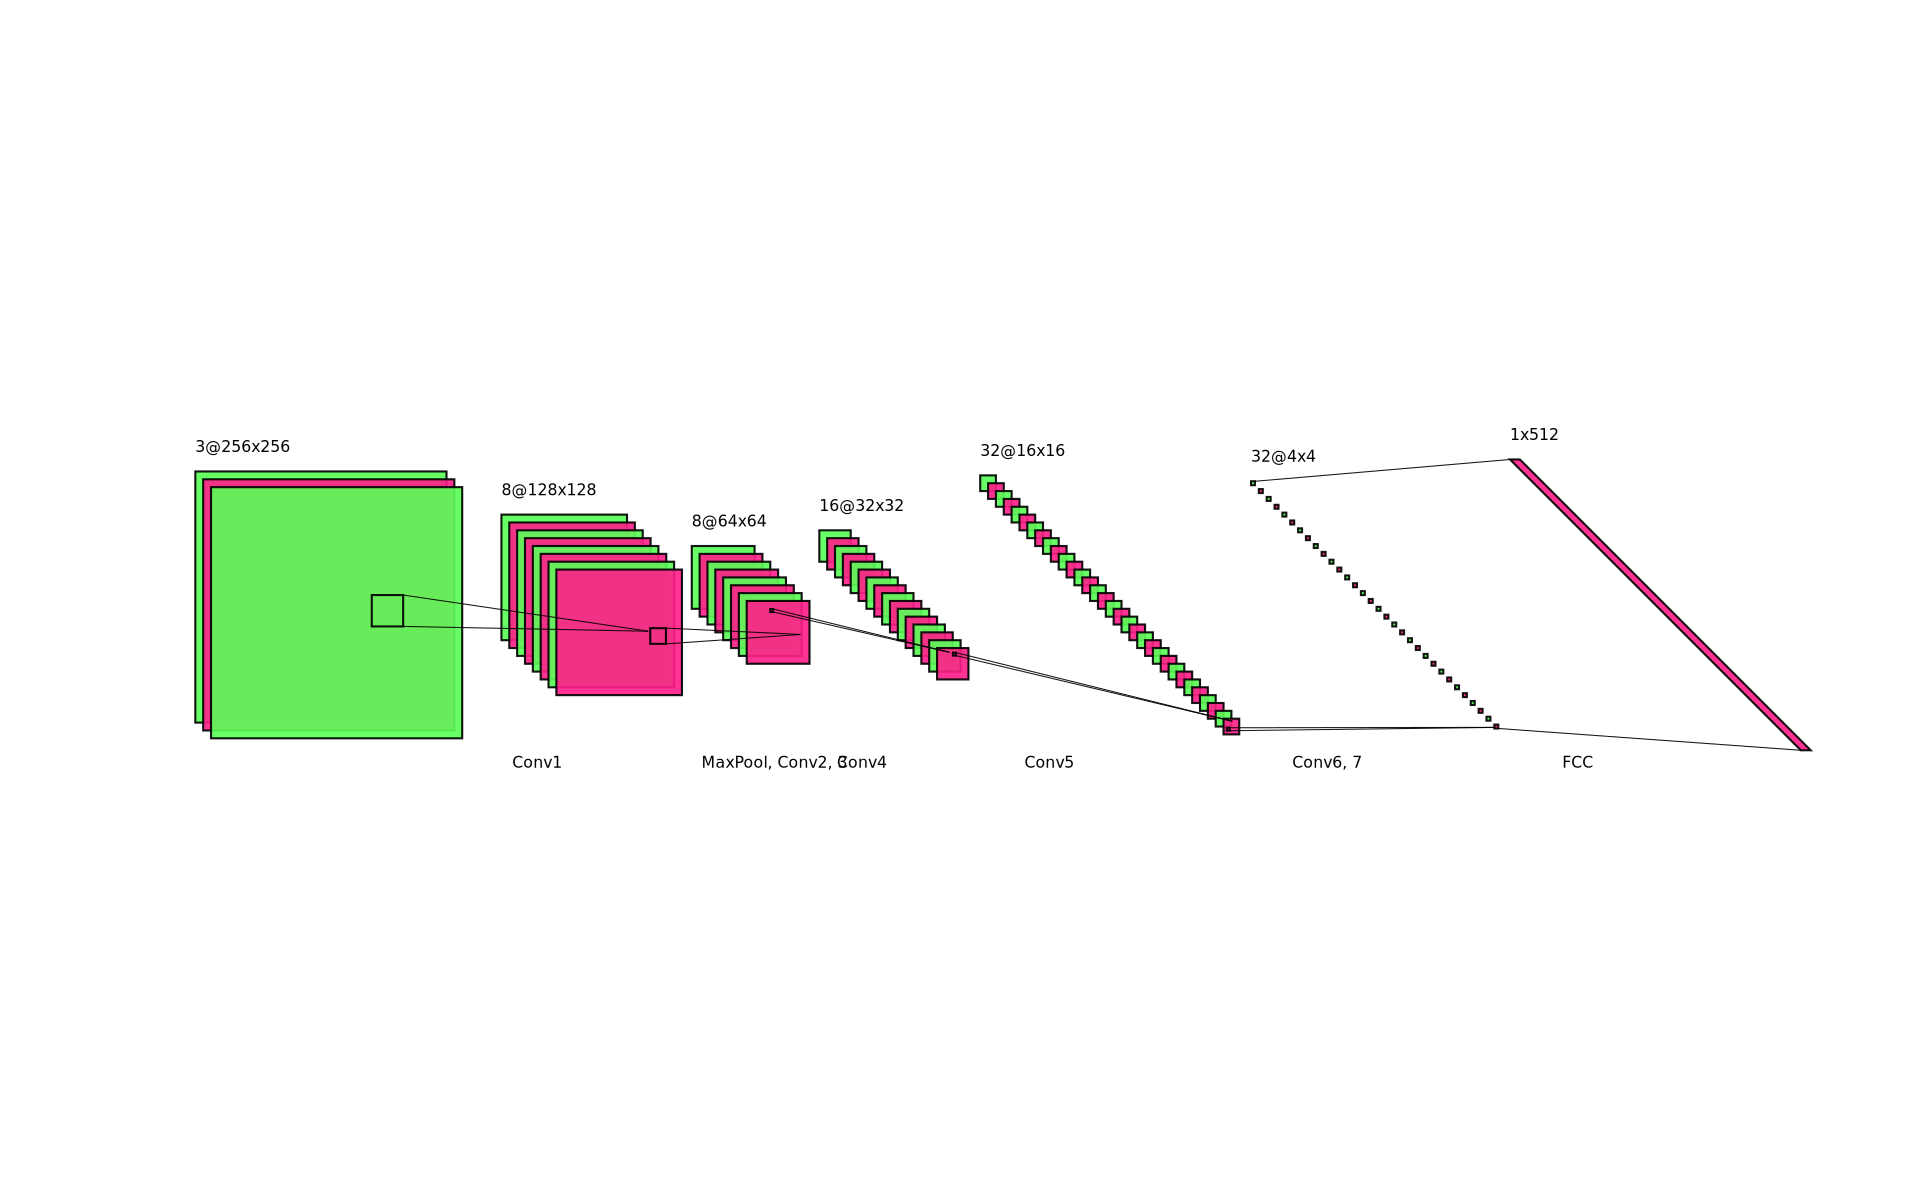
\includegraphics[scale=0.45]{figs/baseline.png}
    \end{center}
    \caption{Baseline model architecture, simplified; the final fully connected layer to a single output neuron.}
    \label{fig:baseline_arch}
\end{figure}

Across various hyperparameter combinations, we observed wide oscillations in our validation curves and overfitting. This is most likely due to the complex nature of the task, which demands greater parameters and epochs than ours. In our best model we were able to achieve a validation accuracy of 67.0\% and a testing accuracy of 65.6\%.

% \begin{table}[t]
%     \caption{Baseline model error statistics; real images are negatives and AI-generated images are positives.}
%     \label{baseline_stats}
%     \begin{center}
%         \begin{tabular}{llllll}
%             \multicolumn{1}{c}{\bf Split} & \multicolumn{1}{c}{\bf Loss} & \multicolumn{1}{c}{\bf Accuracy} & \multicolumn{1}{c}{\bf Precision} & \multicolumn{1}{c}{\bf Recall} & \multicolumn{1}{c}{\bf F1 Score}
%             \\ \hline \\
%             Training                      & 0.303                        & 87.3\%                           & 85.8\%                            & 89.5\%                         & 87.6\%                           \\
%             Validation                    & 0.947                        & 67.0\%                           & 66.2\%                            & 69.6\%                         & 67.8\%                           \\
%             Testing                       & 0.919                        & 65.6\%                           & 64.7\%                            & 68.5\%                         & 66.6\%                           \\
%         \end{tabular}
%     \end{center}
% \end{table}

% \begin{figure}[h]
%     \begin{center}
%         \includegraphics[scale=0.45]{figs/baseline_error_curves.png}
%         \includegraphics[scale=0.45]{figs/baseline_loss_curves.png}
%     \end{center}
%     \caption{Training/validation error (left) and loss (right) curves for the best baseline model.}
%     \label{fig:baseline_curves}
% \end{figure}

\section{Quantitative Results}
\label{quantitative}

The EffViT model achieved a final test accuracy of 85.9\%, which indicates success. As shown in Figure \ref{fig:Training_Curves}, the training versus the validation losses maintain roughly the same value throughout the 30 training epochs. Both begins to plateau around epoch 20, where the training and validation losses reaches 0.2938 and 0.2911, respectively. These correspond to accuracies of 87.79\% and 87.29\%, meaning EffViT is learning the patterns of the embeddings of AI-generated images without over- or underfitting. Detailed statistics of the model can be seen in Table \ref{tab:metrics}.

\begin{figure}[h]
    \begin{center}
        \includegraphics[scale=0.27]{figs/training curves.png}
    \end{center}
    \caption{EffViT's final training and validation loss and accuracy curves.}
    \label{fig:Training_Curves}
\end{figure}

\begin{table}[h]
    \centering
    \caption{Model Performance Metrics}
    \label{tab:metrics}
    \begin{tabular}{lcccc}
        \toprule
        \textbf{Metric} & \textbf{Test Accuracy} & \textbf{Precision} & \textbf{Recall} & \textbf{F1 Score} \\
        \midrule
        \textbf{Value}  & 85.9\%                 & 86.1\%             & 85.56\%         & 85.8\%            \\
        \bottomrule
    \end{tabular}
\end{table}



\section{Qualitative Results}

Section \ref{quantitative} suggests that EffViT performs decently on AI-generated images. However, in the real world, images generated by different architectures/models will exhibit different high- and low-level features. To evaluate how well the model generalizes on images created by different models, four AI-generated images created by distinct models were selected from the test dataset and then passed through EffViT to obtain its output confidence levels.

As shown in Figure \ref{fig:Conf}, EffViT's confidence levels on images generated by GAN-based models are relatively high. On the other hand, EffViT's confidence levels on images generated by DMs and transformer-based models are relatively low. EffViT may be learning subtle artifacts that images generated by GAN-based models have in common. This leads to high confidence on GAN generated images and lower confidence on images that don't contain those artifacts. This biased performance may be caused by an unbalanced training dataset containing more GAN-generated images than diffusion- and transformer-generated images.

\begin{figure}[h]
    \begin{center}
        \includegraphics[scale=0.45]{figs/Confidence shrinked.png}
    \end{center}
    \caption{EffViT confidence levels on images generated by GANs (Cycle-GAN \citep{zhu2020unpairedimagetoimagetranslationusing}, BigGAN \citep{brock2019largescalegantraining}) and non-GAN architectures (Glide \citep{nichol2022glidephotorealisticimagegeneration}, DALL-E Mini).}
    \label{fig:Conf}
\end{figure}


\section{Performance on New Data}

\subsection{Data}

We evaluated our model on three sets of new data: real images from Caltech 256 \citep{griffinholubperona2022}, GAN-generated images from \citet{chuangchuangtanGANGenDetection}, and images generated by diffusion models from \citet{stable-diffusion-100k-custom-prompts-and-images}.

Caltech 256 was chosen for two reasons. First, there were enough images in the set that cropping to 224×224 would not remove too much of the image. Many other datasets with a range of semantics that we considered, for example Open Images \citep{Kuznetsova_2020}, do not contain images small enough for our model. Second, the images in Caltech 256 are very often edited. As shown in Figure \ref{fig:coco_vs_caltech}, many have their background removed, which marks a stark contrast from ImageNet and COCO, where objects are almost always in context. This is more representative of images on the internet, which are often edited, and allows us to evaluate our model for more general use.

\begin{figure}[h]
    \begin{center}
        \includegraphics[scale=0.3]{figs/coco_laptop.jpg}
        \includegraphics[scale=0.45]{figs/caltech_laptop.jpg}
    \end{center}
    \caption{Laptops in context, from COCO (left), and a laptop with no background, from Caltech 256 (right).}
    \label{fig:coco_vs_caltech}
\end{figure}

We used two datasets for AI-generated images because we wanted to evaluate the performance of our model on the two main types of architectures our model was trained on: GANs and diffusion models.

From these datasets, we used 984 real images, and 1,018 fake images, selected at random.

\subsection{Evaluation}

On the new data, our model achieves an accuracy of 74.6\%, and similar precision and recall scores. However, it is much better at identifying images generated by GANs than diffusion models. When only evaluating the GAN-generated dataset, its accuracy is 83.0\%, and when only evaluating the diffusion-model-generated dataset, its accuracy is 59.5\%. This is illustrated in the t-SNE of the hidden activations on the data shown in Figure \ref{fig:new_data_tsne}. We can see that the embeddings of most GAN-generated images form a cluster on the right, whereas most diffusion-model-generated image embeddings are spread throughout the large cluster of mostly real images on the left. However, there is a small cluster of diffusion-model-generated image embeddings at around $(25, -15)$, suggesting the model has learned something about this class of AI-generated images.

\begin{figure}[h]
    \begin{center}
        \includegraphics[scale=0.34]{figs/tsne.png}
        \includegraphics[scale=0.34]{figs/tsne-vit.png}
        \includegraphics[scale=0.34]{figs/tsne-effnet.png}
    \end{center}
    \caption{t-SNE of final model's hidden activations on new dataset, by data type (left), with EffNet neurons zeroed (middle), and with ViT neurons zeroed (right).}
    \label{fig:new_data_tsne}
\end{figure}

Due to the challenging nature of our data as described above, the achievement of our model exceeds our expectations. However, as mentioned in Section \ref{discussion}, we most likely could have improved our model's accuracy on images generated by diffusion models by using training data that was more balanced, relative to images generated by GANs.

\section{Discussion}
\label{discussion}

In our Project Proposal, we presented a somewhat novel zero-shot model for detecting AI-generated images, which involved two steps. The first was a convolutional autoencoder (CAE) which was trained to encode and then reconstruct real images only. Then, it was frozen and given real and AI-generated images, and its pixel-wise reconstruction loss was given to a CNN binary classifier. We were able to train the CAE to a relatively low error, but it performed equally well on both real and fake images, and the classifier performed randomly. Next, we tried replacing the CAE's encoder with a transfer learning model, but again, our classifier gave random predictions. In contrast, the input to EffViT's classifier is the non-decoded embedding. We have learned two things from this: first, that vanilla autoencoders cannot capture the subtle differences between real and fake images, and second, it is the decoder in particular that obfuscates these differences. The output of the decoder is much less useful for this task than the embedding itself.

However, not all embeddings are equal. As mentioned in Section \ref{arch}, ViT and EffNet give us more global and local information, respectively. Figure \ref{fig:new_data_tsne} shows the output of our model's hidden layer, as well as the outputs of that layer, using input neurons from each of ViT and EffNet only. From it, we can make two observations. First, ViT is much better at identifying images from diffusion-based models than EffNet, which essentially cannot tell the difference between them and real images. Second, ViT is much more useful overall; the output of the hidden layer is almost identical to the output of that layer with the EffNet neurons zeroed out. This suggests that our model has learned to discard most of the information EffNet gives it, which implies that global information is much more useful in this problem, especially in identifying diffusion-generated images. Therefore, we speculate that center cropping our images may have removed key information that is needed for this problem.

Other than poor performance on diffusion models, our model's biggest limitation is that its training data does not adequately represent images found ``in the wild''. Images on the internet are often heavily compressed or edited, and our dataset, and especially our synthetic images, do not reflect this reality. Future work should not only use data that is more balanced between synthesis architectures, but also should use data augmentation techniques that represent ``the wild''. These techniques would involve applying lossy compression, such as JPEG, WebP, and HEIF compression, one or more times.

\section{Ethical Considerations}

Our ethical concerns arise from the cases where our model returns false positives and false negatives (a "positive" is a prediction that the image is synthetic). The former could be used to harm artists' and creators' reputations in the case that they are wrongly accused of passing "AI art" as their own work. The latter could be used to spread misinformation, where a malicious actor makes false claims and supports them with "photo evidence", which is in fact fake. We believe our model is especially susceptible to this type of exploitation, due to its performance on images generated by DMs, and our lack of protection against methods such as JPEG artifact analysis. We acknowledge our model's limitations and explicitly disclose that is should be used as an \textbf{assistive tool}, not definitive proof.

\section{Project Difficulty}

This project addressed an \textbf{exceptionally challenging task}: detecting AI-generated images in a landscape where generative models evolve faster than detection tools. Its difficulty proved far greater than what is normally observed in the labs.

As mentioned in the Section \ref{discussion}, we initially aspired to create a zero-shot detector. Due to the challenging nature of the project, it failed and returned random predictions. This presented a challenge for the team, as we had to begin the project with a new perspective. Before arriving at our final EffViT model, we iterated through four intermediate architectures, all of which contained a large amount of trainable parameters. Due to the large amount data used for training combined with the size of these models, we were forced to purchase Google Colab Pro to use A100 GPUs and access additional compute.

No current approach at the moment demonstrates robust generalization to unseen AI architectures \citep{Mubarak2023}. Therefore, we believe our final model does exceptionally well. Not only is its accuracy on new data is still 10\% better than the baseline model's, its accuracy on testing data only 5\% behind many of the SoTA models discussed in Section \ref{background}.

\label{last_page}

\bibliography{APS360_ref}
\bibliographystyle{iclr2022_conference}

\end{document}
